% !TEX root = ../main.tex

% = = = = = = = = = = = = = = = = = = = = = = = = = = = = = =
% = = = = = = = = = = = = = = = = = = = = = = = = = = = = = =

\section{Introduction}

Beginning in the 1980s, a significant amount of the cryptographic literature has been devoted to the design of e-cash systems. In the 1990s, many startups worked toward deployment of this technology but most ultimately failed~\cite{NBFMG16}. By late 2008, when Bitcoin was first proposed, innovation on both the academic and commercial side of digital cash had dried up. Now Bitcoin's success has breathed new life into the field: cryptocurrencies have billion dollar market capitalizations and academic conferences like \textit{Financial Cryptography} are again publishing papers on financial cryptography. 

At first glance, Bitcoin seems like a major departure from the e-cash systems from the 80s and 90s. In reality, its `academic pedigree' is a novel combination of pre-existing ideas~\cite{NaCl17}. Similarly, researchers are re-discovering long lost ideas from the e-cash literature and finding new ways to apply them in a blockchain world. For example, blinded coins were a staple of e-cash~\cite{Cha82} that re-emerge, along with accumulators~\cite{SaTa99}, in post-Bitcoin systems like zcash~\cite{MGGR13,SCG+14}. Enabling micropayments through lottery-based probablistic payments of macropayments was explored in the 90s~\cite{Riv97,Whe97,JaOd97} and re-emerged for Bitcoin~\cite{Pash15}. In this paper, we `re-discover' the 1997 payment system \pw from Rivest and Shamir~\cite{RS96}. 

\pw is a credit-based payment system, envisioned for small payments. The mechanics we will turn to later, but for now, the reader can think of tokens being issued that have some value. The key limitation of \pw is that tokens do not have inherent value; their value is based on the trust assumption that a counter-party will honour the value ascribed to them. With Ethereum and other blockchain technologies, we can fix this issue by stapling cryptocurrency to the token through the use of a smart contract. 

This transformation turns \pw from a trust-based credit system to a escrow-based payment system; not unlike offline payment channels and networks being proposed for Bitcoin --- the Lightning Network being the most prominent~\cite{PD15}. After presenting our system, \ew, we discuss its relation to payment channels. It is known that an Ethereum-based payment channel will be less complex than a Bitcoin one, since most of the complexity of Bitcoin-based payments channels (\eg \textblue{setup is XX transactions and payment is YY}~\cite{MMSH16}) comes from Bitcoin's limited scripting language. \ew a uni-directional (monotonic) payment channel that can be chained into a payment network and has very compact (\eg 112-bit) payments. It thus might be an interesting primitive to enhance in the same ways other payment channels~\cite{DW15,PD15} have been: adding features~\cite{KG17}, increasing efficiency~\cite{DEFM17,MBKM17}, and adding transactional privacy~\cite{GM17,MMK+17,HAB+17,RMKG18}.

% = = = = = = = = = = = = = = = = = = = = = = = = = = = = = =
% = = = = = = = = = = = = = = = = = = = = = = = = = = = = = =

\section{Preliminaries}

\subsubsection{Hash Chains}

A hash chain is constructed by iteratively applying a public one-way hash function $\Hash{}$ on a random value $s$. Let the notation $\HashN{i+1}{s} = \Hash{\HashN{i}{s}}$. A hash chain of length $n+1$ is:
\begin{equation*} \tuple{s,\Hash{s},\HashN{2}{s},\HashN{3}{s},\ldots,\HashN{n-1}{s},\HashN{n}{s}} \end{equation*}

where $s$ (technically equivalent to $\HashN{0}{s}$) is called the \textit{seed} and $\HashN{n}{s}$ is called the \textit{tip}. Given the hash is preimage resistant against a computationally bounded adversary, knowing some value in the chain $\HashN{x}{s}$ does not reveal any values `up' the chain from it, including the seed: $\tuple{s,\ldots,\HashN{x-1}{s}}$. Conversely the value $\HashN{x}{s}$ can be iteratively hashed to produce the rest of the values `down' the chain ending up producing the tip value. 

\subsubsection{Message Recognition}

One application of a hash chain is a message recognition protocol. If Alice meets Bob at a party, Bob can give the tip of a chain to Alice as a token. Later when Bob meets Alice again, he can provide $\HashN{n-1}{s}$ as proof he is the the same person that gave her the token. On the subsequent visit, he provides $\HashN{n-2}{s}$ and so on for $n$ visits. Of course, Bob could more directly provide Alice with his public key and sign messages each visit, however hash chains avoid the relatively expensive public key operations of a signature scheme. 

\subsubsection{Payments}

In \pw, a hash chain is used for credit-based payments. A customer generates a length $n+1$ hash chain and provides a signed tip to the merchant. They agree that each preceding value in the hash chain has a specified unit of value owed to the merchant by the customer. For example, say $n$ is 100 and the value of each hash in the chain is a \$1 debt owed to the merchant. To expense \$27, the customer provides $\HashN{n-27}{s}$ to the merchant who will verify that hashing it 27 times produces the signed tip. The customer can increase the amount by sending further hashes, up to \$100 (after which, the payment channel is \textit{exhausted} and must be reinitiated).

% = = = = = = = = = = = = = = = = = = = = = = = = = = = = = =
% = = = = = = = = = = = = = = = = = = = = = = = = = = = = = =

\section{\ew}

\ew is an Ethereum-based smart contract that enables the aggregation of an offchain set of small payments to one or more onchain larger transactions. Particularly, our contract implements a smart contract moderated version of the Payword micropayment protocol and mediates the interaction between a customer $C$ and a merchant $M$. A pseudocode for the proposed smart contract is shown in Figure \ref{fig.contract}. 

%\begin{figure}[!th]
%	\centering
%	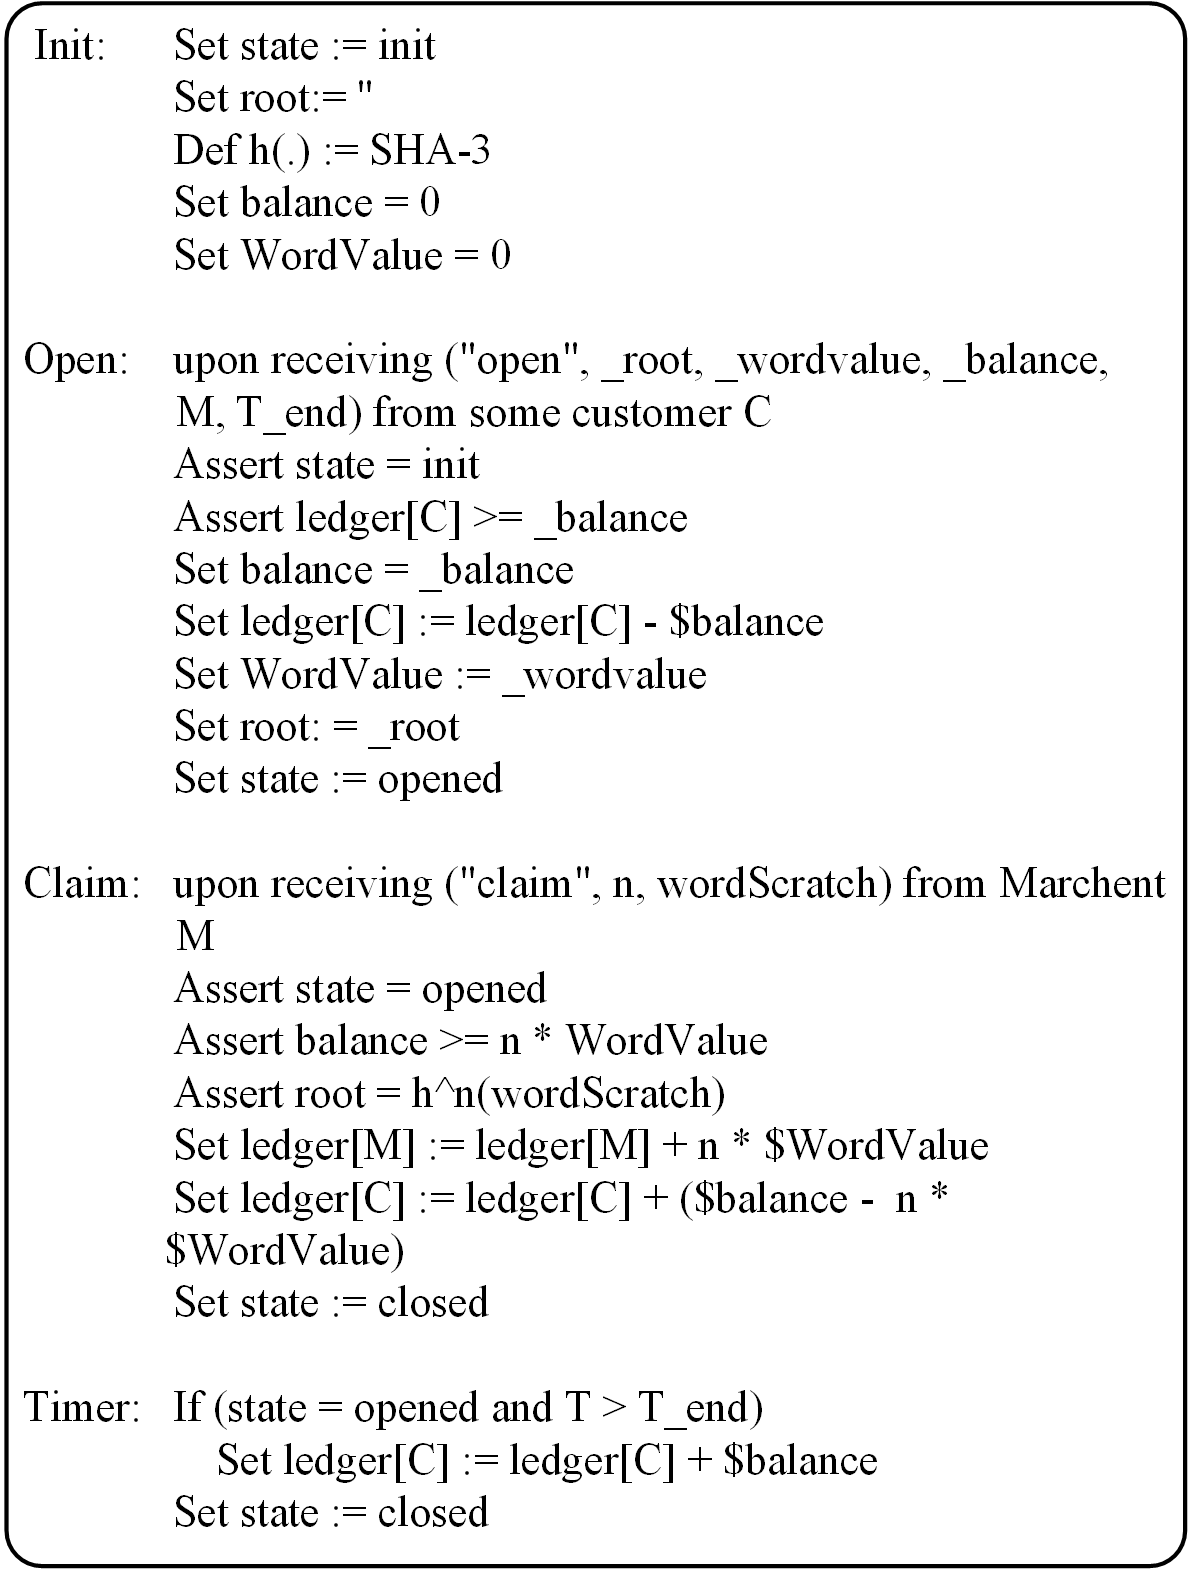
\includegraphics[scale=0.7]{pics/contract.png}
%	\caption{A pseudocode for the proposed \ew smart contract.}
%	\label{fig.contract}
%\end{figure} 

EthWord is designed with two main functions that mediate the transaction process between $C$ and $M$. First, the contract is instantiated by $C$ through calling the \texttt{open} function. In this function, $C$ initializes the contract through passing the pseudonym of the merchant's account $M$, the tip of the hash chain $\_root$ so that the contract can verify released intermediate hash values against it, the amount that each released hash value is worth $\_wordvalue$, and the total amount of the whole hash chain $\_balance$, and $T_{end}$ which is the time after which remaining funds in the contact's balance are refunded to the customer's account. After calling the \texttt{open} function, both the contract and merchant can evaluate the length of the chain and, thus, $M$ can offline know how many intermediate hash values she can accept from $C$ without the need to constantly monitor the state of the contract. Also, $M$ knows that she has to claim aggregated payments before $T_{end}$ or else, $M$ can refund the contract's available balance.

\subsection{Claiming aggregated payments} 

For each payment in the form of an intermediate hash $x=h^i(s)$, $i=1,2,\cdots,N-1$ that $M$ receives from $C$, she can verify its validity offline by evaluating if $h^{(N-i)}(x) = h^N(s)$ or not. Accordingly, $M$ can decide whether to accept the transaction or decline it in the event of a failed verification. After a few micropayments, where $M$ has acquired a set of intermediate hashes, she invokes the \texttt{claim} function in the smart contract by passing to it the last received hash value $wordScratch$, and its order within the hash chain $n$. Consequently, the contract verifies the validity and the required balance of the supplied inputs against the stored hash chain parameters, and upon successful verification, the account of $M$ is credited by the resulting balance.

\subsection{Payment networks} 

\subsection{Efficiency}

\subsection{Security}

EthWord smart contract provides the following guaranteed security properties:
\begin{itemize}
	\item Fair exchange of services:
	\item Conducting irrefutable transactions without blockchain monitoring:
\end{itemize}

% = = = = = = = = = = = = = = = = = = = = = = = = = = = = = =
% = = = = = = = = = = = = = = = = = = = = = = = = = = = = = =

\section{Relation to Payment Channels}

% = = = = = = = = = = = = = = = = = = = = = = = = = = = = = =
% = = = = = = = = = = = = = = = = = = = = = = = = = = = = = =

\section{Discussion}


















